\documentclass[letterpaper,twocolumn,amsmath,amssymb,pre]{revtex4-1}
\usepackage{graphicx}% Include figure files
\usepackage{color}

\newcommand{\red}[1]{{\bf \color{red} #1}}
\newcommand{\blue}[1]{{\bf \color{blue} #1}}
\newcommand{\green}[1]{{\bf \color{green} #1}}

\newcommand{\fixme}[1]{\red{[#1]}}
\newcommand{\davidsays}[1]{{\color{red} [\green{David:} \emph{#1}]}}
\newcommand{\renesays}[1]{{\color{red} [\blue{Rene:} \emph{#1}]}}
\newcommand{\jeffsays}[1]{{\color{red} [\blue{Jeff:} \emph{#1}]}}

\newcommand\micron{\ensuremath{\mu\text{m}}}

\begin{document}
\title{Robustness of MinD oscillation in \emph{Escherichia coli} with
  diverse cell shapes}

\author{Jeff B. Schulte}
\affiliation{Department of Physics, Oregon State University}
\author{Rene W. Zeto}
\affiliation{Department of Physics, Oregon State University}
\author{David Roundy}
\affiliation{Department of Physics, Oregon State University}

\begin{abstract}
  The dynamics of the Min-protein system help Escherichia coli
  bacteria regulate the process of cell division by identifying the
  center of the cell.  We model the Min-protein system in bacteria
  that have been forced into unusual flattened shapes, as have
  recently been experimentally observed.  We find that although the
  presence of Min oscillations is robust in a wide variety of cellular
  configurations, the location of the peaks is strongly affected by
  the cellular shape.  In some cases no periodic oscillations are
  observed.  In particular, we find that cellular shapes observed
  experimentally to present irregular oscillations do so in the
  theoretical model, consistently \fixme{or inconsistently?} with
  experiment.  \fixme{In agreement with previous theoretical and
    experimental results, we observe ``rotating'' behavior in certain
    shapes having three corners.}
\end{abstract}

\maketitle

\section{Introduction}
It is vital that during the process of bacterial cell division a cell
avoid minicelling, or splitting into daughter cells with lopsided
volumes.  Instrumental to this process in \emph{Escherichia coli} is a
long FtsZ polymer chain that develops on the cell wall in the center
region of the cell, helping dictate the plane of
division~\cite{adams2009bacterial, lutkenhaus2007assembly}. Previous
experimental studies have shown that the MinC protein, known to
inhibit the FtZ polymer\cite{shen2010examination}, exhibits pole to
pole oscillatory behavior in conjunction with the MinD protein and a
MinE that tends to be more localized in the center of the
cell~\cite{hu1999topological, fu2001mine, shapiro2009and, yu1999ftsz,
  raskin1999rapid}. The MinC protein will then have a higher time
averaged concentration in the cell poles, as opposed to the center
region of the cell, aiding in prohibiting the FtZ from developing in
the wrong region.

Studies have shown that the cell division process is capable of
preventing minicelling for fairly perturbed cell
shapes\cite{touhami2006temperature}. Varma et al. studied one
particular example of a perturbed shape, a three-pronged tube, and
found both experimental and simulation results\cite{varma2008min} that
show oscillation. These oscillations seem to seek out the extreme
poles in the cell shape\cite{corbin2002exploring}
\cite{juarez2010changes}, and effectively prevent minicelling in most
cases. However, Mannik et al. have also shown that there are
limitations to this mechanism\cite{mannik2010bacteria}
\cite{mannik2009bacterial}. One instance of this behavior is
observable when the cell has been forced into a flattened, irregular
shape. Oscillations in this sort of cell shape are far from the
regular sorts of oscillations seen in the computational work done by
Huang et al\cite{huang2003dynamic}. We seek to apply a computational
model to explore the more extreme or irregular cell shapes, in order
to determine the limits of the steady cell oscillations seen by both
theory and experiment.

A significant amount of work has been done to develop protein reaction
and diffusion models that exhibit accurate macroscopic dynamics of the
MinD protein system. Early models involve free proteins that affect
each others' rates of diffusion and membrane attachment, but do not
combine into compound states~\cite{meinhardt2001pattern}.  In 2003
Huang improved upon this work with a simple simulation model based on
MinD-MinE combination, ATPase hydrolysis, and MinD membrane attachment
that exhibits accurate MinD oscillations in
cylindrical cells~\cite{huang2003dynamic}. In this model cytoplasmic
MinD is more likely to attach to the membrane when MinD is already
clustered there (following observed non-linear attachement of minD on
the cell membrane), and is stationary once attached.  A number of
studies have used an approach similar in that they do not rely on the
ability of MinD to move along the walls and
cluster~\cite{kruse2007experimentalist, meinhardt2001pattern,
  drew2005polymerization, fange2006noise, kerr2006division}, while
studies have been made as well of models which rely on MinD mobility
and attraction on the cell membrane~\cite{kruse2002dynamic,
  howard2005cellular}.  Variations of the Huang 2003 model that
stochasticly account for variations of molecular interaction
\cite{fange2006noise} and monte-carlo simulations that implement this
stochastic version of Huang's mean field reaction rates confirm the
major results obtained by Huang's model, and more successfully predict
experimentally observed oscillations in round cell
phenotypes~\cite{drew2005polymerization, fange2006noise,
  huang2004min}. Biochemical models of broader scope have also been
used to study the MinD system and show consistent
results.\cite{arjunan2010new}.  However, in general, the results of
the stochastic and monte-carlo simulations are similar to those given
by Huang's mean field results.

Previous studies have been made of the Min system's associtation with
the cell membrane
\cite{hsieh2010direct}\cite{mileykovskaya2003effects}.  Studies have
shown as well that MinD binds preferentially to regions enriched with
cadiolipin, an anionic phospholipid that collects on regions of high
negative curvature. This mechanism has been incorporated into other
models.\cite{drew2005polymerization,cytrynbaum2007multistranded,renner2012mind,renner2012mind}
However, this mechanism of combined clustering, phospholipids and MinD
has not been observed in real cells. \cite{halatek2012highly}


\begin{figure}
  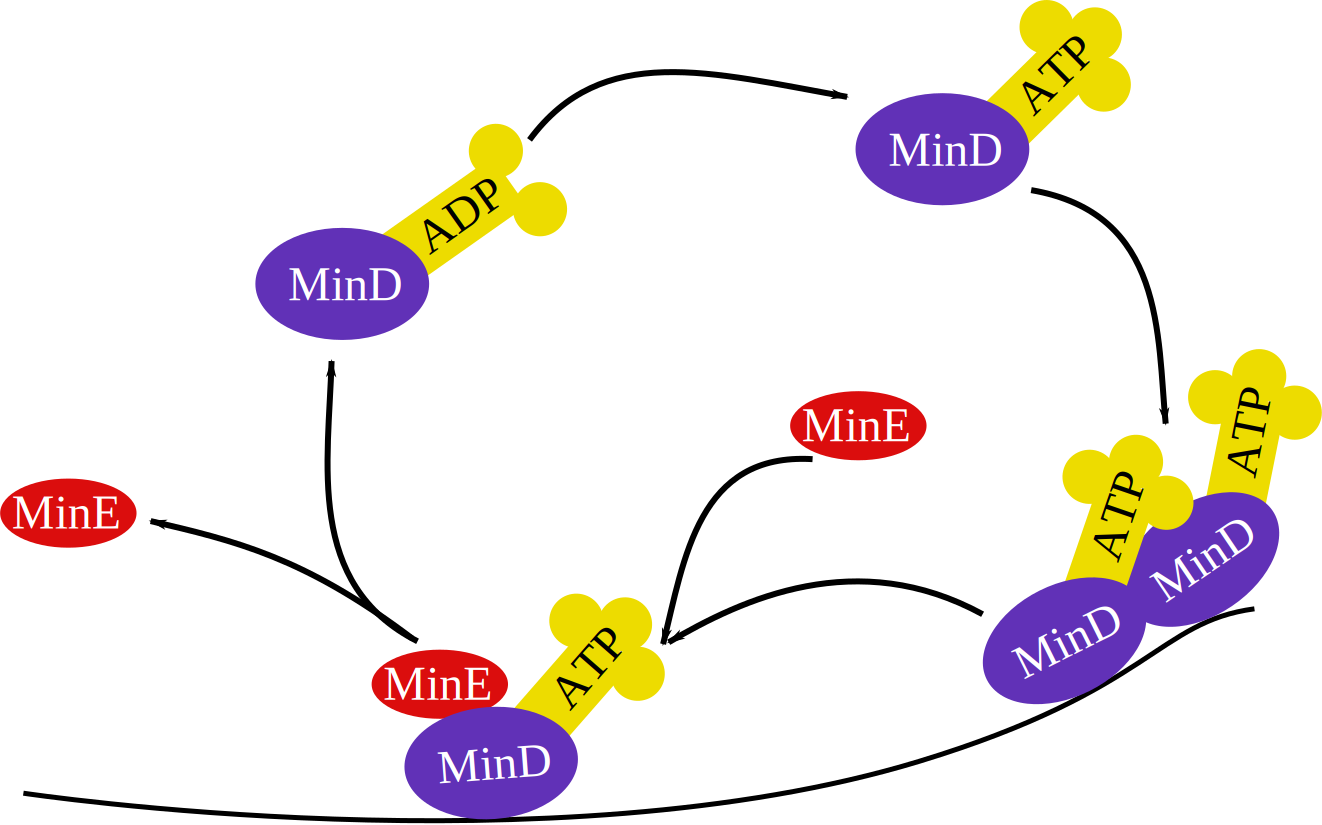
\includegraphics[width=\columnwidth]{reactions}
  \caption{Reactions included in the model of Huang \emph{et
      al.}~\cite{huang2003dynamic}.}\label{fig:reactions}
\end{figure}


\section{Model, Methods, and Pill Shaped Cell}
We implement the model of Huang \emph{et al.}  for the behavior of the
MinD and MinE proteins inside the cell~\cite{huang2003dynamic}.
Figure~\ref{fig:reactions} shows the reaction process.  The
cytoplasmic MinD:ADP complex undergoes nucleotide exchange and is
changed into the MinD:ATP complex.  This will naturally diffuse
towards and attach to the cell membrane.  A cytoplasmic MinE will
attach to the wall bound MinD:ATP complex and after a time will
activate ATP hydrolosis.  This breaks up the complex, releasing MinE,
phosphate, and MinD:ADP back into the cytoplasm.  The MinD:ADP will undergo
nucleotide exchange and begin again the cyclic process.  This model is
defined by a set of five reaction-diffusion equations:

\begin{multline}
  \frac{\partial \rho_{D:ADP}}{\partial t} = \mathcal{D}_D\nabla^2\rho_{D:ADP}-k_D^{ADP\rightarrow ATP}\rho_{D:ADP}\\
  +\delta(d_w)k_{de}\sigma_{DE},\hspace{3.4cm}
\end{multline}
\begin{multline}
  \frac{\partial \rho_{D:ATP}}{\partial t} = \mathcal{D}_D\nabla^2\rho_{D:ATP}+k_D^{ADP\rightarrow ATP}\rho_{D:ADP}\\
  -\delta(d_w)[k_D+k_{dD}(\sigma_D+\sigma_{DE})]\rho_{D:ATP}
\end{multline}
\begin{multline}
  \frac{\partial \rho_E}{\partial t} = \mathcal{D}_E\nabla^2\rho_E+\delta(d_w)k_{de}\sigma_{DE}
  -\delta(d_w)k_E \sigma_D \rho_E
\end{multline}
\begin{multline}
  \frac{\partial \sigma_D}{\partial t} = -k_E\sigma_D\rho_E
  +[k_D+k_{dD}(\sigma_D+\sigma_{DE})]\rho_{D:ATP}
  \label{eq:d-on-wall}
\end{multline}
\begin{multline}
  \frac{\partial \sigma_{DE}}{\partial t} = -k_{de}\sigma_{DE}+k_E\sigma_D\rho_E\hspace{3cm}
  \label{eq:FifthPDE}
\end{multline}

where $\rho$ is cytoplasmic protein density ($\mu m^{-3}$), $\sigma$
is membrane bound density ($\mu m^{-2}$), $\mathcal{D}_D$ and
$\mathcal{D}_{E}$ th diffusions constants for MinD and MinE,
respectively, $k_D^{\textrm{ADP $\rightarrow$ ATP}}$ the rate of
conversion from MinD:ADP to the MinD:ATP complex, $k_D$ the rate of
MinD:ATP attachement to the membrane when no protein is already
attached there, $k_{dD}$ the increase of this rate when MinD:ATP is
present on the membrane, $k_{de}$ the rate of hydrolisis of the
MinD:MinE:ATP complex, $k_E$ the rate of cytoplasmic MinE binding to
membrane bound MinD:ATP complex, and $d_w$ is the distance from the
point in space to the closest wall (which will always be
perpendicular to this distance).  $\delta(d_w)$ has units of
$\mu m^{-1}$ and will be zero everywhere except at the wall.
Equations \ref{eq:d-on-wall} and \ref{eq:FifthPDE} will only be
relevent at the membrane because the membrane bound density values
will have no meaning in the cytoplasm where there is no membrane.

Our diffusion and reaction rates are shown below.  We are interested
primarily in the effect of cellular size and shape on the protein
oscillations, so we follow Huang\cite{huang2003dynamic} and do not
deviate from the wild type values used in the cited work (see values
below).  Huang's simulations use total MinD and MinE concentrations of
$1,000/\mu m$ and $350/\mu m$, respectively, in a cylindrical cell of
radius $0.5\mu m$, and in our (non-cylindrical) cells we use the same
number of proteins per unit volume.  These concentration values are
1273 $\mu m^{-3}$ and 446 $\mu m^{-3}$, respectively.
\begin{gather*}
  \mathcal{D}_D = \mathcal{D}_{E} = 2.5\micron^2/\text{sec}\\
  k_D^{\textrm{ADP $\rightarrow$ ATP}} = 1/\textrm{sec,  }
  k_D = 0.025 \micron /\textrm{sec}\\
  k_{dD} = 0.0015 \micron^3/ \textrm{sec,  }
  k_{de} = 0.7/\textrm{sec}\\
  k_E = 0.093 \micron^3 /\textrm{sec}.
\end{gather*}
A 3D grid is then constructed in cartesian coordinates, with a grid
spacing of .05\micron.

In order to further our understanding of the results of various
simulation approaches to this system, we have performed both a basic
finite analysis, deterministic simulation that is spatially and
temporally discrete, and a stochastic analysis that is spatially
discrete but continuous in time.  Our stochastic simulation method
follows the work of Kraus~\cite{kraus1996crosstalk} which in turn
follows a method introduced by Gillespie~\cite{gillespie1977exact}.

We mean to investigate the geometric limits of the Min system
oscillations as observed by Mannik \emph{et
  al.}~\cite{mannik2012robustness}, so we model the Min system in a
variety of cell shapes and sizes.  Here we present a selection of
those, first naturally occuring pill-shaped cells and then a
number of flattened out shapes which reflect the experiments of Mannik
\emph{et al.}, in which bacteria are confined within a thin slit of
height $0.25\micron$ ~\cite{mannik2012robustness}. Viewed from the top
down the cells will have the shapes described below and viewed from
the side they have at their edges a semicircular protrusion (one may
imagine the edges of a pancake). Central to our observations are the
effects of cell size and so we show expanded cells that have the same
thickness but increased dimensions in the two planar directions.  We
present two shapes that are designed to replicate those published by
Mannik, equilateral and iscosolese triangle shapes, and a 'V' shape of
our own creation in order to best illustrate the effect of cell size
on oscillation stability.

%% Our pill shapes differ from those of Huang \emph{et al.} in that they
%% are cylinders with hemisphere endcaps instead of pure cylindrical
%% shapes.  Our cylinderidrical radius is $0.5\micron$ and the lengths
%% of our cells (measured between the tips of the endcaps) are
%% $5\micron$, $4\micron$, $3\micron$, and $2.5\micron$.

Kubitschek has shown in multiple experiments that at the time of cell
division cells have a volume that is within a range of roughly
$1\micron^3$ to $2\micron^3$~\cite{kubitschek1990cell,
  kubitschek1968linear}.  We follow Huang's
simulations\cite{huang2003dynamic} and Mannik's experiments and model
cells that are slightly larger than this range.

\begin{figure*}
  \includegraphics[width=\textwidth]{../data/shape-p/plots/image-plot--p-300-50-0-0-1500-exact}
  \includegraphics[width=\textwidth]{../data/shape-p/plots/single-image-plot--p-300-50-0-0-1500-full_array}
  \caption{Countour plot images of the concentration of each protein
    species in a natural pill-shaped bacterium at regular intervals in
    time (one second intervals), with darker regions indicating higher
    concentration. The upper plots shows results from the
    deterministic simulation and the lower shows results from the
    stochastic simulation.  The cells pictured are $4\micron$ in
    length, measured from end to end.  The order of frames is such
    that individual MinD proteins begin at the bottom of the plot (in
    the MinD:ATP state in the cytoplasm), and progress upward until
    they reach the MinE:MinD:ATP membrane-bound complex.  At that
    point, they will spontaneously dissociate into cytoplasmic MinE
    (the top row) and the starting state of cytoplasmic MinD:ADP.  The
    densities plotted are integrated along the axis orthogonal to the
    page, and the color scale is chosen separately for each species
    with black as the maximum value over space and time.  The
    stochastic densities are smeared out over space using a guassians
    approximation developed by Zhang et all~\cite{zhang2007gaussian}}.
  \label{image-p}
\end{figure*}

We begin with the naturally occuring pill cell shape.  We peice this
shape together as two hemispherical endcaps attached on either end of
a cylinder.  This shape follows the early simulations of Huang
\emph{et al.} but differs in that we have added the end caps for a
more natural shape, expecting similar results.  We test cells of
radius $.5\micron$ and of lengths $2\micron$, $3\micron$, and
$5\micron$ measured from the tip of one end cap to the tip of the
other. In each case, we observe in the deterministic simulations a
quick establishement (within a few periods) of extremely regular
oscillatory behavoir that lasts indefinitely.  The stochastic results
show oscillitions that are similarly regular in time, with periods
that nearly match those of the deterministic (they differ roughly by a
factor of .05). The stochastic results also show a slight variation in
the height of the density maxima, but the peaks are still very well
defined. The period increases with cell length, as shown in
Table~\ref{tab:pill-periods}, in agreement with the results of Huang
\emph{et al.}.  The stochastic simulations show a similar pattern.
The MinD maxima occur at the ends of the cell in a back and forth
manner, and with the same approximate period.

\begin{table}
  \begin{tabular}{|r|c|c|c|l|}
    \hline
    Length($\mu$) & 2.50 & 3.00 & 4.00 & 5.00\\
    \hline
    Period(sec) & sim & 33 & 38 & 48 \\ \cline{2-2}
    \hline
  \end{tabular}
  \caption{Period of oscillation according to length of cell for
    pill-shaped cells.}\label{tab:pill-periods}
\end{table}

This simple cell shape is a good starting point for observing in
detail the dynamic interaction between the different stages of protein
that lead to their qualitatively distinct behavoir. Figure
\ref{image-p} shows the process in a series of frames taken from
simulation animations for both the deterministic and stochastic
simulations.  We have 'smeared out' the stochastic concentrations in a
manner meant to reproduce the images shown by diffraction limited
flourescence microscopy.  We do so using the two dimensional gaussian
approximation developed by Zhang et all~\cite{zhang2007gaussian}.  In
this approximation we use a numerical aperture value of 1.3, which is
the same as used by mannik experimentally, and a wavelength of
$509nm$, typical of green flourescent microscopy.  Each frame is 2.5
seconds ahead of the last, and each image shows a the concentration of
a given state of protein summed over the coordinate orthogonal to the
page.  The color scale for each protein state is set according to the
maximum values observed.

At $t=0$ in Figs.~\ref{image-p}, the cytoplasmic MinE is concentrated
in the lower portion of the cell and is diffusing upward, since it
will react with and stick to wall-bound MinD that is concentrated on
the membrane in the upper portion of the cell.  At the boundary
between the cytoplasmic MinE and the membrane-bound MinD, there is a
ring of the membrane-bound MinE:MinD complex, which is moving towards
the upper end of the cell, removing the MinD from the membrane as it
goes.  The MinD is removed from the membrane in its MinD:ADP form and
diffuses freely for a time before spontenously undergowing nucleotide
exchange and shifting back into the MinD:ATP that is able to attach to
the membrane.  Diffusion away from the end of the cell will bring the
protein into the MinE ring, where reactions will prevent it from
collecting for any significant time on the membrane.  Diffusion
further towards the upper end, however, while the MinE has not yet
collected there, will allow MinD:ATP to accumulate with the other
MinD:ATP, peaking at around 10 seconds in Figure~\ref{image-p}.  As
the MinE ring approaches the end of the cell, seen in the seconds
following 10, the only freely diffusing MinD:ADP that 'escapes' the
MinE will be that which has diffused away from the the end of the cell
and past the MinE ring towards the center.

At 15 seconds, the membrane-bound MinD:ATP has been essentially
removed from the top end of the cell, and MinD:ATP has begun to bind
to the membrane in the the lower half of the cell.  At this stage,
there is a high concentration of cytoplasmic MinE at the top of the
cell, and by 16 seconds we begin to see the formation of a MinE ring
just below the center of the cell.  At 18 seconds, the cell has
reached its original state (reversed directionally), with MinD:ATP
bound to the membrane on the lower third of the cell, a high
concentration of cytoplasmic MinE in the upper half of the cell, and a
MinE ring pushing downward on the membrane-bound MinD:ATP.

\begin{figure}
  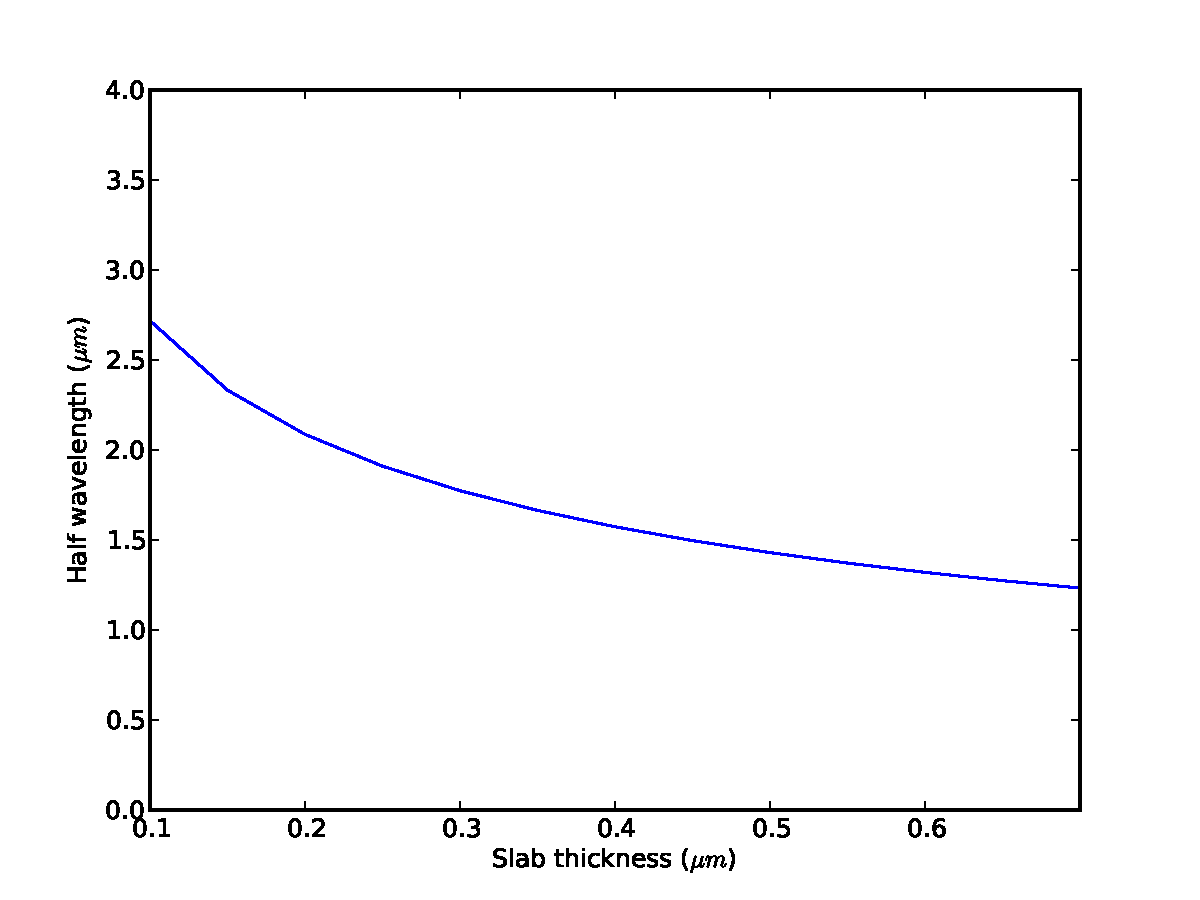
\includegraphics[width=\columnwidth]{stability-analysis}
  \caption{Infinite slab stability analysis yields characteristic half
    wavelengths at which system becomes unstable.}
    \label{fig:stability-analysis}
\end{figure}


\section{Stability Analysis}
We have found that in both methods of simulation there is a lower
length scale that characterizes much of the behavoir.  Regular
oscillatory behavoir between two poles at opposite ends of the longer
cellular direction is found in cells which are long enough in one
dimension for the reaction chain to be unstable but short enough in
the perpendicular dimension to be stable.  The limits are seen when
both dimensions are too short to be unstable, so that initial
assymetry in protein concentration relaxes into a state of no
oscillation.  In these cell sizes, the deterministic simulations show
a motionless steady state and the stochastic simulations show random
fluctuations without any bulk behavoir (see Figure~\ref{box-mannik}).

In order to explain this theoretically, we have performed stability
analysis of the five differential equations in an infinite slab that
show a characteristic half wavelength in perturbative spatial
oscillations at which the system becomes unstable.  This length is
dependent upon slab thickness as shown in
Figure~\ref{fig:stability-analysis}.  When increasing the lengths and
widths of our simulated flattened cells, the cells stop exhibiting two
pole oscillalitory behavior and instead exhibit multiple positions of
maximization when the shortest distance across the cell is
approximately equal to the characteristic half wavelength at the
particular thickness at which we simulate (our simulations of cells
with thickness $0.25\mu m$ corresponds to half wavelengths of $2.13\mu
m$).  Huang~\cite{huang2003dynamic} performs a similar analysis for a
cylindrical shape \fixme{is it cylindrical or 1d?} and finds
characteristic half wavelengths of $2\mu m$.

\begin{figure}
%  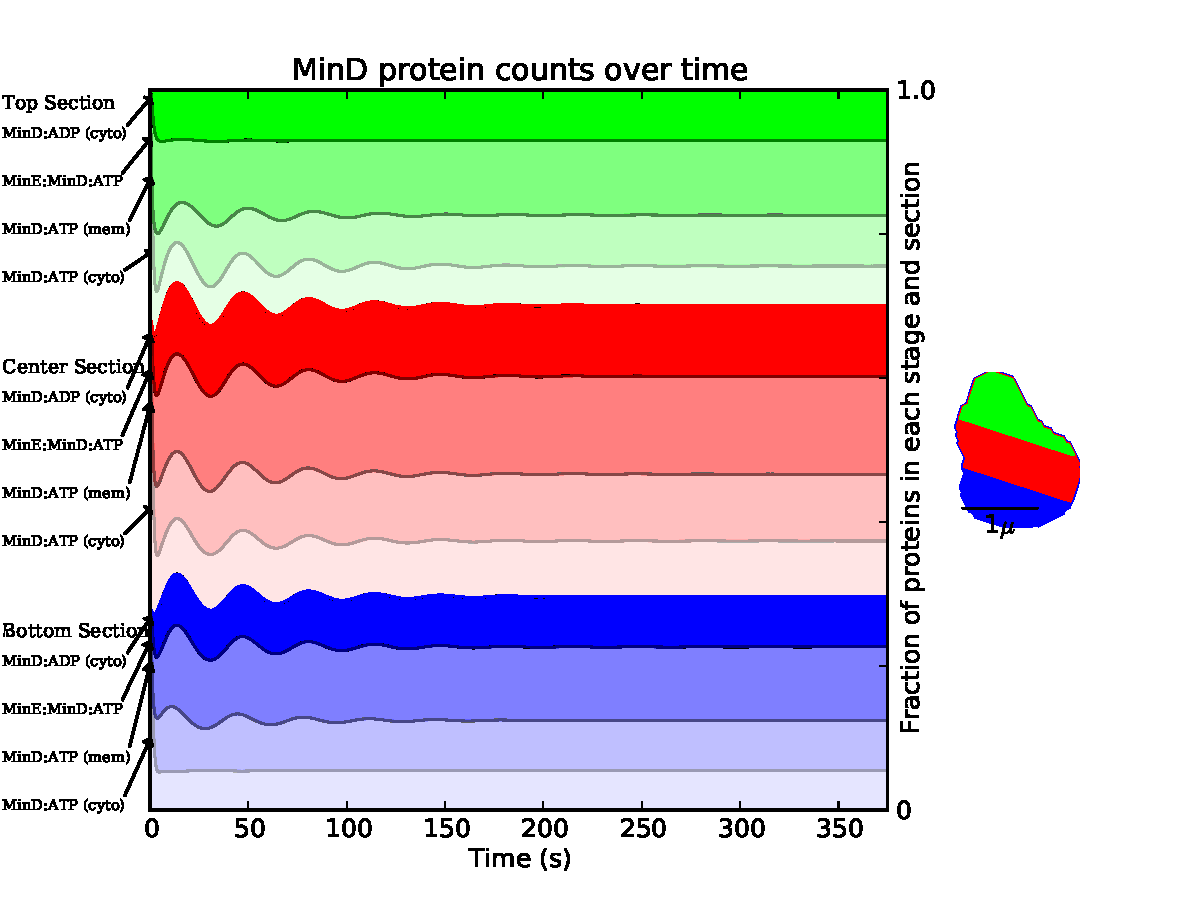
\includegraphics[width=4.2cm]{../data/shape-randst/plots/box-plot_D--randst-25-800-800-9500-1500}
%  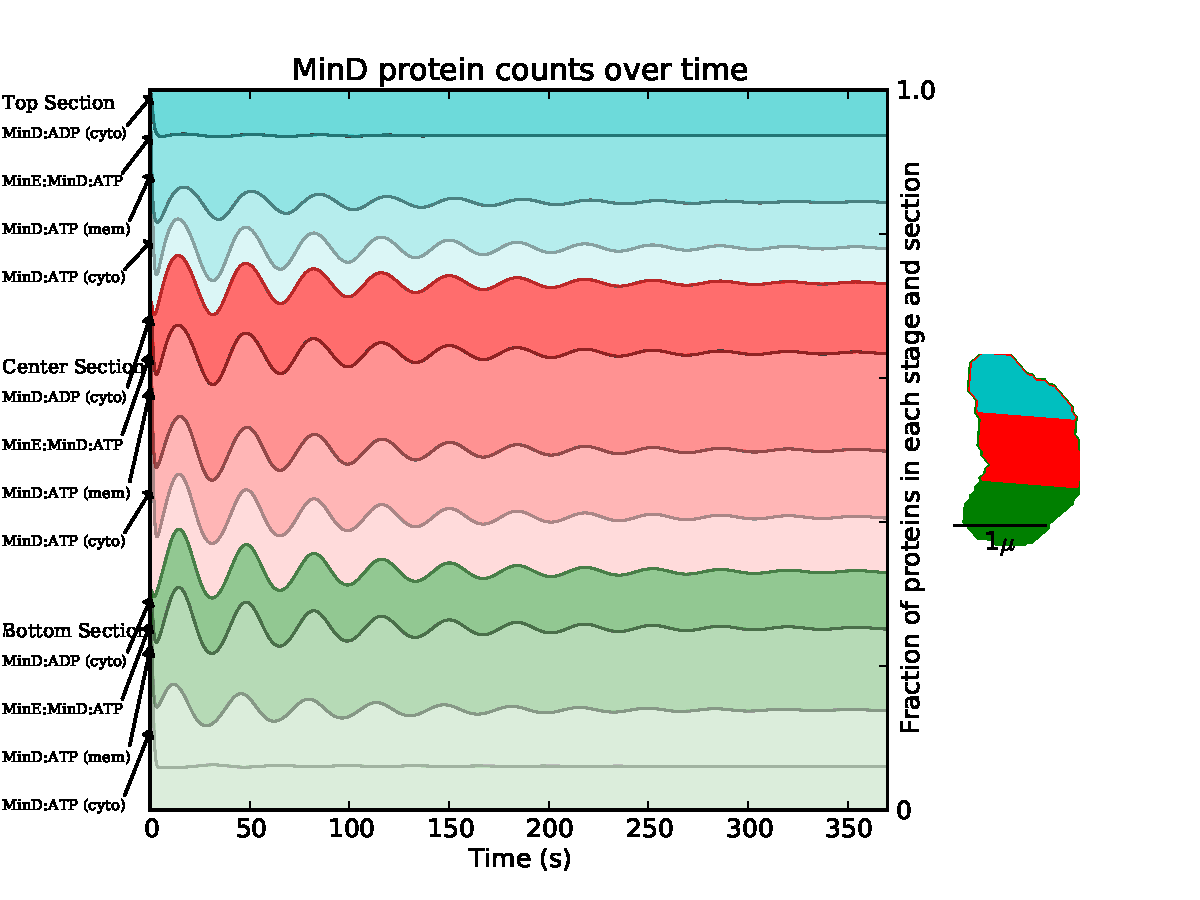
\includegraphics[width=4.2cm]{../data/shape-randst/plots/box-plot_D--randst-25-1000-1700-9400-1500}
  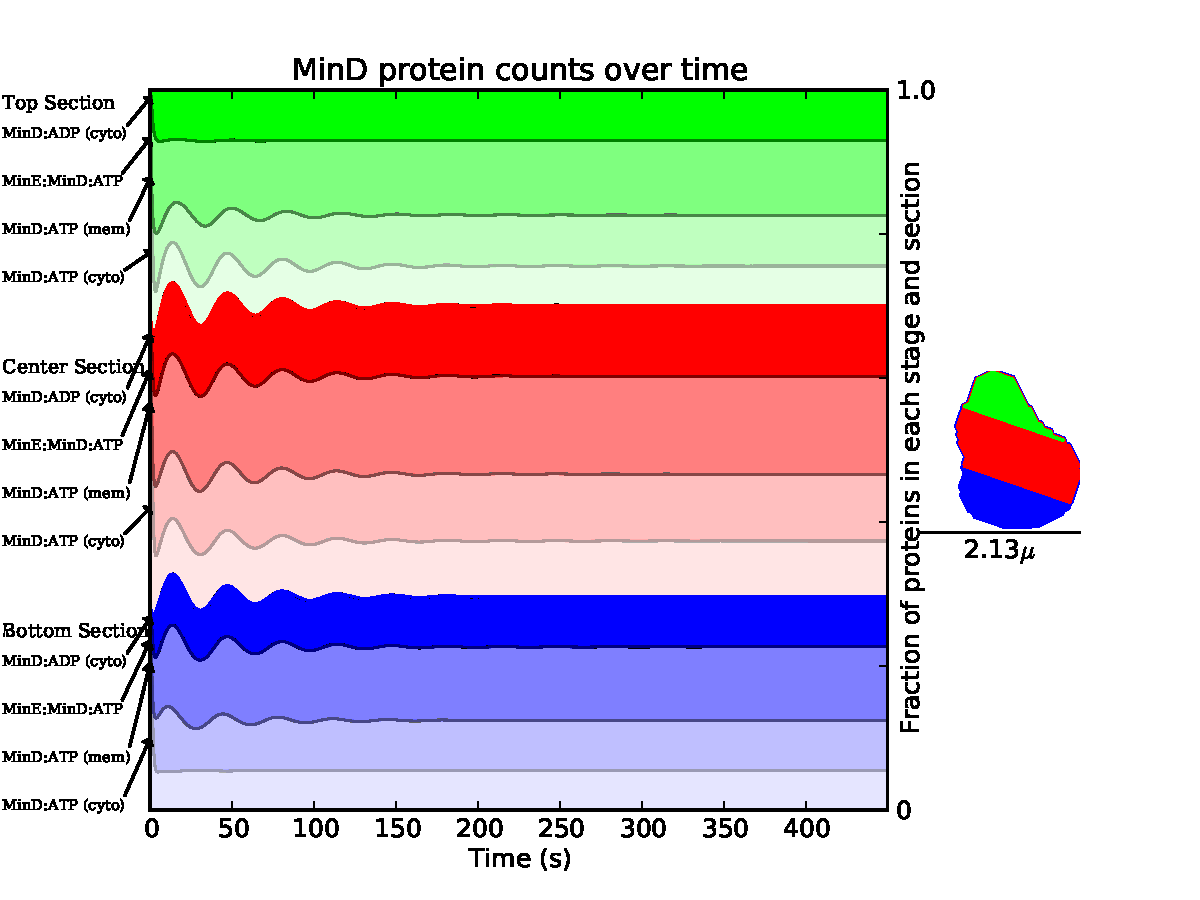
\includegraphics[width=\columnwidth]{../data/shape-randst/plots/box-plot_D--randst-25-800-800-9500-1500-exact}
  \includegraphics[width=\columnwidth]{../data/shape-randst/plots/box-plot_D--randst-25-1000-1700-9400-1500-exact}
  \caption{Box plots of Mannik shapes for sizes at the lower stability
    threshhold.  The vertical axis shows stacked and changing over
    time the total number of proteins that are of four different
    compound stages and in the different sections of the cell.  Both
    shapes have longer axis of roughly 2.2$\mu m$.}
  \label{box-mannik}
\end{figure}

Decreasing the cell size in succesive steps, we can see the critical
size at which the cell oscillations are quickly damped out.
Figure~\ref{box-mannik} shows box plots of the largest cells simulated
whose oscillations relax into the steady state solution.  Both have a
long axis of roughly 2.2$\mu m$, in agreement with theory.

%% \begin{figure}
%%   \includegraphics[width=\columnwidth]{../data/shape-randst/plots/paper-arrow-plot}
%%   \caption{Arrow plots for our simulation and mannik's experimental}
%%   \label{arrow-compare-mannik}
%% \end{figure}

\section{Comparison of Mannik's Experimental and Our Stadium Shapes}
In general we have found that the deterministic simulations of the
protein reaction sequence discussed above results in robust
oscillatory behavoir of polar selection and oscillation in a wide
variety of cell shapes.  On the other hand, the stochastic simulations
show back and forth behavoir that breaks down in more assymetric
shapes with larger sizes, which is similar to what Mannik has observed
experimentally.

\begin{figure}
  \includegraphics[width=\columnwidth]{../data/shape-stad/plots/plot-time-averaged-arrow-500-520-NflD-stad-25-400-150-0-1500-full_array}
  \caption{Arrow plots of our stadium shape}
  \label{stadium-arrow}
\end{figure}

\begin{figure}
  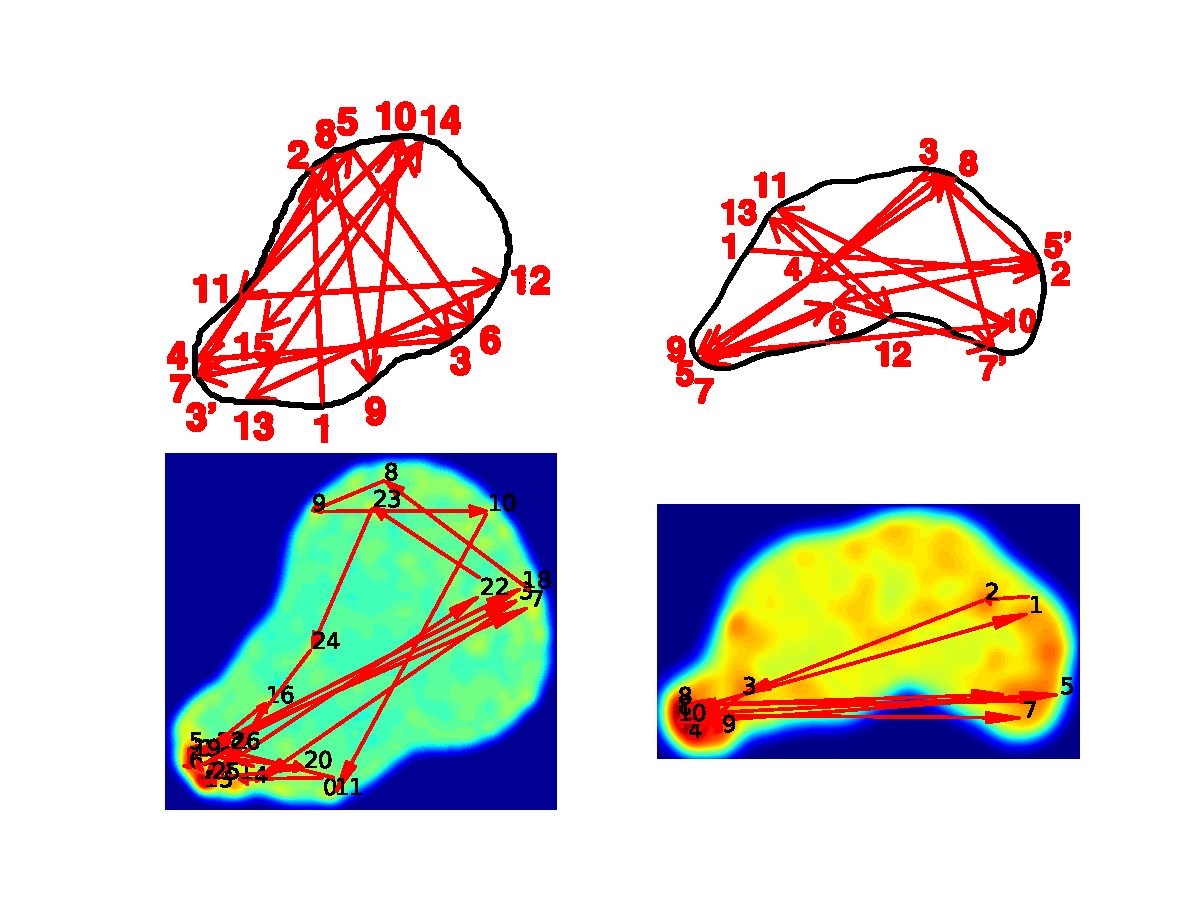
\includegraphics[width=\columnwidth]{../paper/plot-ave}
  %% \includegraphics[width=\columnwidth]{../data/shape-randst/plots/arrow-1500-95-stoch}
  %% \includegraphics[width=\columnwidth]{../data/shape-randst/plots/arrow-1850-95-stoch}
  %% \includegraphics[width=\columnwidth]{../data/shape-randst/plots/arrow-2500-95-stoch}
  \caption{Arrow plots of our randst shape}
  \label{stadium-arrow}
\end{figure}


\begin{figure}
  \includegraphics[width=\columnwidth]{../data/shape-stad/plots/time-map-NflD-stad-25-600-200-0-1500-full_array}
  \includegraphics[width=\columnwidth]{../data/shape-stad/plots/time-map-NflD-stad-25-400-150-0-1500-full_array}
  \caption{Time map plots of our stad shape}
  \label{time-maps-stad}
\end{figure}


\begin{figure}
  \includegraphics[width=\columnwidth]{../data/shape-randst/plots/time-map-NflD-randst-25-1850-1850-9500-1500-full_array}
  \includegraphics[width=\columnwidth]{../data/shape-randst/plots/time-map-NflD-randst-25-2500-2500-9500-1500-full_array}
  \includegraphics[width=\columnwidth]{../data/shape-randst/plots/time-map-NflD-randst-25-1860-2860-9400-1500-full_array}
  \includegraphics[width=\columnwidth]{../data/shape-randst/plots/time-map-NflD-randst-25-2300-3200-9400-1500-full_array}
  \caption{Time map plots of our randst shape}
  \label{time-maps-randst}
\end{figure}


\fixme{specifically design other arrow plot (with many comparisons) to
  illustrate point}


Figure~\ref{arrow-compare-mannik} shows plots of total MinD
concentration maxima that are global in space and local in time.  The
tip of an arrow represents one of these maxima and the adjacent arrow
(whose tail is touching the previous arrow's tip) points to the next
such maxima in time.  Mannik \emph{et al.} have published similar
plots of two of their cells, and we have attempted to replicate the
shape of these cells in our simulation in order to compare.  We find
that when we replicate the size as well as shape of their cells as
near as possible, we do not see the disordered protein behavoir that
they observe.  Instead we see a robust ability of the cell to find two
prefered pole locations and to oscillate maxima back and forth very
steadily between them.  When we increase the size of our cells, we
indeed see multiple positions of maxima develop, but we never observe
the random behavoir that they have observed experimentally.  This is
perhaps due to the exact, continuous method we use when conducting
simulations.  Stochastic methods would perhaps show more random
behavoir at these sizes.  We consider this to be a limitation of the
exact solution method.

%% \section{Triangular Shapes}

%% \begin{figure}
%% %  \includegraphics[width=4.2cm]{../data/shape-triangle/plots/box-plot_D--triangle-25-233-233-233-1500}
%% %  \includegraphics[width=4.2cm]{../data/shape-triangle/plots/box-plot_D--triangle-25-266-266-266-1500}
%%   \includegraphics[width=\columnwidth]{../data/shape-triangle/plots/box-plot_D--triangle-25-233-233-233-1500}
%%   \includegraphics[width=\columnwidth]{../data/shape-triangle/plots/box-plot_D--triangle-25-266-266-266-1500}
%%   %\includegraphics[width=4.2cm]{../data/shape-triangle/plots/box-plot_D--triangle-25-800-800-800-1500}
%%   \caption{Two box plots of triangle shapes.  The two smaller show
%%     sizes at the lower stability threshhold, one just below, one just
%%     above.  The larger triangle is the largest simulated. The vertical
%%     axis shows stacked and changing over time the total number of
%%     proteins that are of four different compound stages and in the
%%     different sections of the cell.}
%%   \label{box-triangle}
%% \end{figure}

%% Along with our other shapes we have chosen to simulate both
%% equilateral and iscoscolese triangular flattened shapes, since these
%% offer in a way the simplest shapes that are geometrically more
%% complicated than our pills.

%% Both triangle types show a similar oscillation pattern.  The
%% iscosolese exhibit regular oscillations characterized by one distinct
%% pole in the more accute angle of the three, and another 'pole' along
%% the opposite wall, peaking in the two more obtuse angles at the same
%% time.  The equilateral triangles settle very quickly into the same
%% pattern, where the choice of which is one pole corner is dependent
%% upon initial conditions.  As with the Mannik simulated shapes, there
%% is a critical small size below which the oscillations dampen out and
%% will not achieve a regular pattern.  Figure~\ref{box-triangle} shows
%% two plots of equilateral triangles.  The two smaller show the
%% largest that showed damped out behavoir and the smallest that
%% developed regular oscillations.  The larger shows the largest traingle
%% that we simulated, showing that at even very large sizes the behavoir
%% is consistent and stable.  Above the small size threshold, all
%% simulated triangles show regular patterns for as long as simulated
%% (roughly 800 seconds).



%% \section{Our '\textgreater' Shaped Cells}
%% \begin{figure}
%%   \includegraphics[width=\columnwidth]{../data/shape-randst/plots/box-plot_D--randst-25-525-525-9900-1500}
%%   \includegraphics[width=\columnwidth]{../data/shape-randst/plots/box-plot_D--randst-25-550-550-9900-1500}
%%   \label{fig:Vbox}
%% \end{figure}
%% \begin{figure}
%%   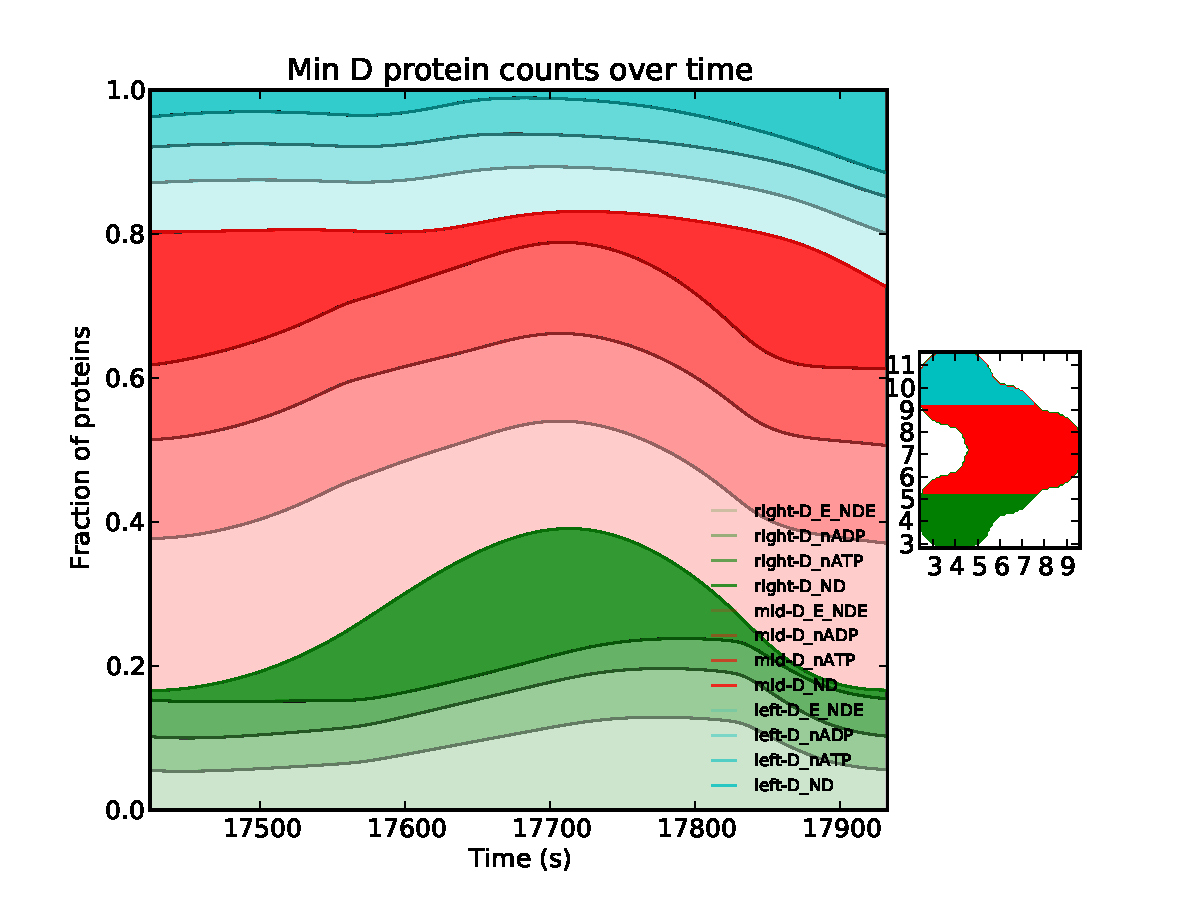
\includegraphics[width=\columnwidth]{../data/shape-randst/plots/box-plot_D--randst-25-600-600-9900-1500}
%%   \includegraphics[width=\columnwidth]{../data/shape-randst/plots/box-plot_D--randst-25-1400-1400-9900-1500}
%%   \label{fig:Vbox2}
%% \end{figure}

%% We have also simulated a flattened '\textgreater' shape that shows an
%% interesting size dependent pattern (seen in
%% Figures~\ref{fig:Vbox}~and~\ref{fig:Vbox2}).  When the shape is small enough
%% that the distance from the apex tip to the opposite curve is less than
%% our stability limit, a simple, two pole oscillation pattern develops
%% and is sustained (where the two poles are on opposite leftward corners
%% of the cell).  When the cell is increased in size so that this
%% distance is approximately equal to our stability value, the cell
%% develops a double oscillation in time, where the maxima oscillates
%% from the lower corner to the rightward apex, then \emph{back to the
%%   lower corner}, then to the apex again, then to the upper corner,
%% then back to the apex, then to the upper corner, then to the apex
%% again, then back to the lower corner, and continues this pattern
%% indefinately.  Figure~\ref{fig:Vbox} shows the smaller size, for which the
%% protein oscillates simply, and an intermediate size, which shows a
%% pattern for which one out of three spikes in the regular oscillation
%% is less significant.  This second pattern seems to be a precursor to
%% the double oscillation that seen in Figure~\ref{fig:Vbox2}.  The second
%% plot shown in Figure~\ref{fig:Vbox2} shows a slightly larger cell for
%% which the distance measured is larger than our stability limit
%% distance.  This simulation shows a random pattern.

%% A detailed analysis of a time series of protein contour plots shows
%% that the importance of spatial dimensions is based on the ability of
%% protein in different stages to diffuse neccesary distances before
%% undergowing certain types of reactions.  The double oscillation
%% pattern shows that every time the membrane bound MinD maximizes in the
%% upper corner as opposed to the rightward apex, it does so because the
%% MinE has not had enough time to diffuse to this upper corner, leaving
%% a MinE free zone.  This particular pattern is specific to this shape
%% and size, but in general its the restrictions set in place by the
%% rates at which proteins diffuse and the distances they cover before
%% reacting that dictate their oscillatory bahavoir.

%% Simulations of this shape in which the two planar dimensions are large
%% compared to those shown(roughly $9\micron$ across) show no stable
%% regular periodic pattern. Animations show that the MinD acts as a sort
%% of traveling cluster that is constantly being eaten away by MinE
%% behind it.  When this cluster enters a region of high curvature that
%% ends in a dead end corner it performs the polar maxima behavoir seen
%% in the other simulations, regrouping out away from the corner where it
%% travels in the opposite direction while being ``chased'' away by the
%% MinE that itself is currently maximizing in the corner.  The maxima
%% occur on non-polar walls often, and will often split into two roaming
%% clusters.



\section{Interpretation of Data}
\section{Conclusion}
\bibliography{paper}



\end{document}

\section*{Appendix}

\section{Below are NOTES for the Writing}

Figure \ref{total-oscillation-triangle-plot} shows the equivalent
motion and transference between compound states for the triangular
states as Figure \ref{total-oscillation-plot} does for the pill shaped
cells.  The equilateral triangular shows that in all three sections
there is a spike in wall attached MinD-ATP directly followed by a
spike in wall attached MinD-MinE-ATP.  The pill had shown a similar
pattern except that the mid section exhibited no such pronounced
spike.  Interestingly, the right and mid sections show spikes at
similar times when compared to the left section spikes, which seem to
oscillate in a manner shifted pi off from the other two.  This
behavoir shows itself in the animations, which show a relaxation into
a stable oscillation from a maxima in one corner to a double maxima in
the other two corners, and back again.  The left section heights are
roughly twice that of the right section heights.  The simulations are
started with higher concentrations of proteins in primarily the right
section, with some overlap into the middle section, so that perhpas
this oscillation pattern seems reasonable.  However, it's interesting
to note that the oscillations, started with assymmetric density, do
not naturally rotate around the corners of the triangle in a circular
pattern.


It seems as well that there is a desired oscillation maxima for the
particular shape and size of the cell, as can be seen by the
relaxation, over the first four periods, to a regular maximal height
of the right and left sections' total protein at the height of each spike.

\fixme{Note to make sure I'm interpreting the iscosolese triangle data
  correctly: the triangle sides are 5,5,3, and the higher density
  starts in the corner that is opposite the short side.  This corner
  is covered by the right section.  I've verified this by looking at
  the protein\_microscopy and drawing a little picture, which is on my
  desk...if you dare look for something on my desk!!!}  The iscosolese
triangle starts its simulation with a higher concentration of protein
in the section that is opposite the shorter side.  It quickly relaxes
into a stable oscillation pattern.  This pattern shows that right
corner section regularly has higher spikes in total protein than the
other sections, and that its spikes appear one pi removed from the
spikes for the other two sections.  This a similar behavoir to that
which is seen in the equilateral triangle, differening in that it
converges more quickly towards this behavoir and that it shows a
greater exageration in the height of protein buildup in the right most
section.

\fixme{Note on interpretation of 3-4-5 triangle: the higher density
  starts to the right of a vertical line that is parrallel to the
  second longest side in the triangle (the longer of the two
  non-hypotonuse sides).  This means the higher concentration covers
  the right angle and also the smaller angle in the triangle} The
3-4-5 triangle exhibits behavoir that I need more data to properly
observe.  I does not converge as quickly as that for the iscosolese or
equilateral triangles.


It seems that there is an approximate critical cell size for which the
MinD will act in these ``wandering cluster'' formations.  The cell is
large enough so that there is a loss of MinD correlation between the
opposite sides (the protein in the right corner at any time is too far
away from the left to immediately affect the protein there).


\fixme{running larger and smaller.  Guessing the larger will do pole
  and pole, so talk about in terms of you have huge, pole and pole,
  then once get small enough double oscillations develop.  Why do they
  do that?  And hen you can do image plot for the one with consistent
  double oscillations.  Can right now explain reason for double
  oscillations.  Look at todo.txt.  The slightly varied guassian shape,
  so a little assymetric, doesn't change double oscillation pattern.}

Contour plot frames from the animations show the second maxima in the
lower left corner (immediately following the one in the upper middle
corner) will reside for a bit longer than the left corner maxima
preceding it.  These longer residing maxima will then be followed by a
switch, to the right corner, with a short, less intensive maxima
traveling through the center.  The MinE shows the same pattern. The
MinE that was just concentrated on the left corner during the first
maxima, after releasing the MinD from the membrane there, diffuses up
and attaches to the MinD on the upper corner membrane and begins to
release it.  During this process the MinE starts at the edges and
moves in towards the center of the maxima.  The center of the cup is a
little further away so it attaches to these outer ridges first and
then moves in.  After it eats at the corners and starts moving in the
MinD eventually travels back to set up a maxima in the left corner.
Watching the cytoplasmic MinE, something very interesting: It as well
maximizes twice in the left corner, but during the MinD's first maxima
in the left corner, the MinE has a maxima in the upper corner, and
during the MinD's second left maxima, the MinE travels to the right
corner and has a maxima there.  At the same time (during the second
MinD left corner maxima), there is a large amount of cytoplasmic
MinD:ATP on the right side.  The MinE does this becuase during the
first MinD left corner maxima, the MinE has just come off a maxima in
the right corner.  So it diffuses up to the upper corner and sets up
there.  During the second MinD left corner maxima, the MinE has just
come off the upper corner maxima.  It will diffuse into the right
corner and left corner.  In the left corner it interacts with the MinD
bound to the membrane there.  In the right corner it sits and
eventually diffuses away, but at a somewhat slow pace.  \fixme{An idea
  is that once the MinD travels back from the left corner after its
  second maxima there, it is not able tot set up a maxima in the upper
  corner as easily, since there is left over MinE there, which has
  just traveled from the right corner.  The problem with this is that
  the MinE doesn't seem to be maximized in the upper corner when the
  MinD is traveling back up from the left.}  The other idea is simply
that because the minE is traveling all the way from the right corner,
the longer time it takes to get there simply means that it all
concentrates on the left, leaving the upp and right side completely
open for the build up of MinD.  \fixme{Still dont quite get it but
  take a look at the other simulations and come back.} Actually, you
can see this effect very slightly watching the 98 shape, between the
center cap and the right corner.

Simulations of this shape that has the same height and dimensions .6
times the size (cells roughly $1.6\mu m$ from top to bottom) do not
exhibit the same pattern.  In these the MinD maxima oscillate quickly
back and forth between the two lower corner poles.

Simulations in which the two planar dimensions are 2 and then 3 times
the size (cells roughly $6\micron$ and $9\micron$, respectively, from top
to bottom) show no stable regular periodic pattern \fixme{although
  they haven't really run long enough to exhibit much.  They certainly
  won't show the double oscillation pattern, however.}  The animations
of $6\micron$ cells show that the MinD acts as a sort of traveling
cluster that is constantly being eaten away be MinE behind it.  When
this cluster enters a region of high curvature that ends in a dead end
corner it performs the polar maxima behavoir seen in the other
simulations, regrouping out away from the corner where it travels in
the opposite direction while being ``chased'' away by the MinE that
has itself maximized in the corner.  If it has just maximized in the
top corner, it regroups traveling downward and then naturally splits
into two groups that travel out and form maxima in the two opposite
bottom corners.  After maximizing in these two corners the two groups
recombine again in the center and travel in some direction together as
one cluster.  Simulations of the $9\micron$ cells show a similar roaming
cluster.  Although here, the maxima occur on non-polar walls often,
and will often split into two roaming clusters that interact less
quickly and are less correlated than those seen in the $6\micron$ cell.

It seems that there is an approximate critical cell size for which the
MinD will act in these ``wandering cluster'' formations.  The cell is
large enough so that there is a loss of MinD correlation between the
opposite sides (the protein in the right corner at any time is too far
away from the left to immediately affect the protein there).


%% \subsubsection{Randst-97-}
%% \begin{figure}
%%   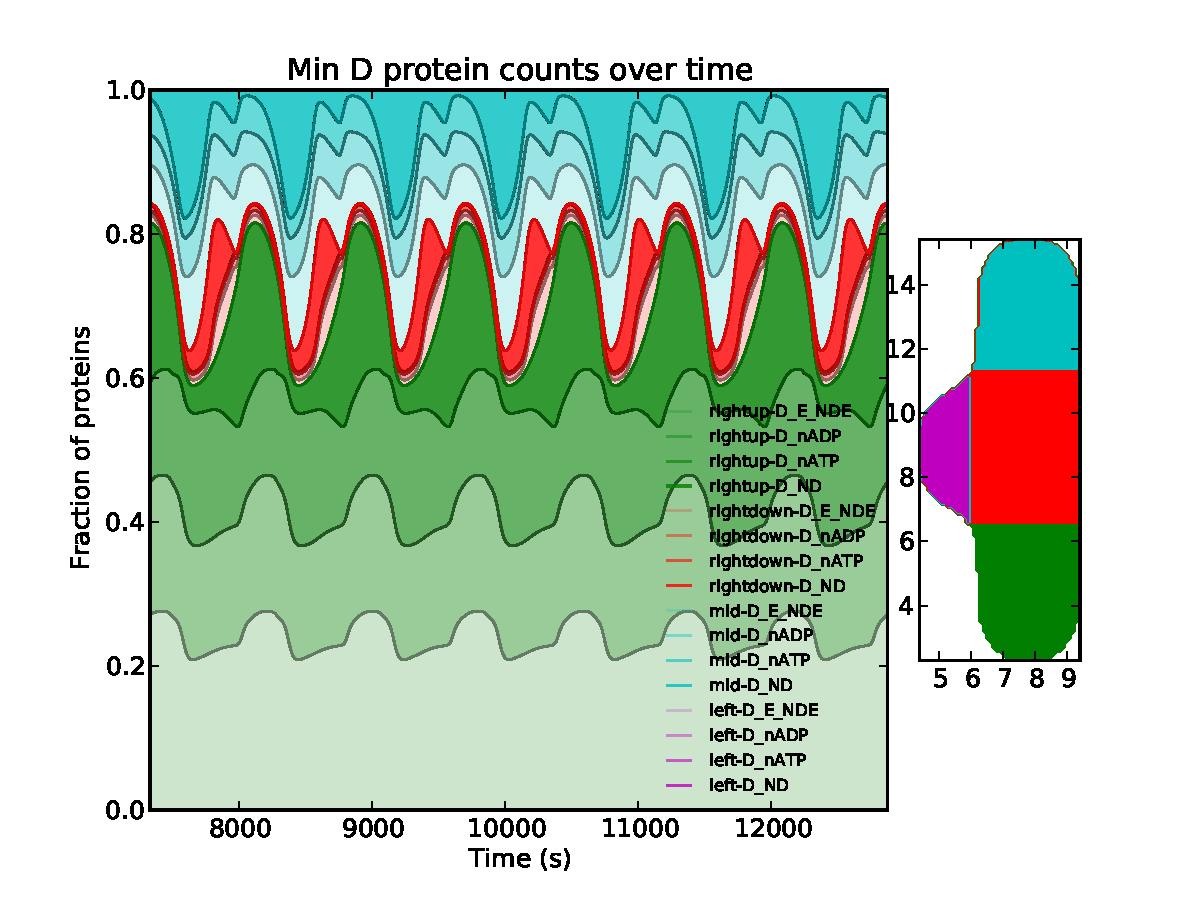
\includegraphics[width=\columnwidth]{../data/shape-randst/plots/box-plot_D--randst-25-800-600-9700-1500}
%%   %%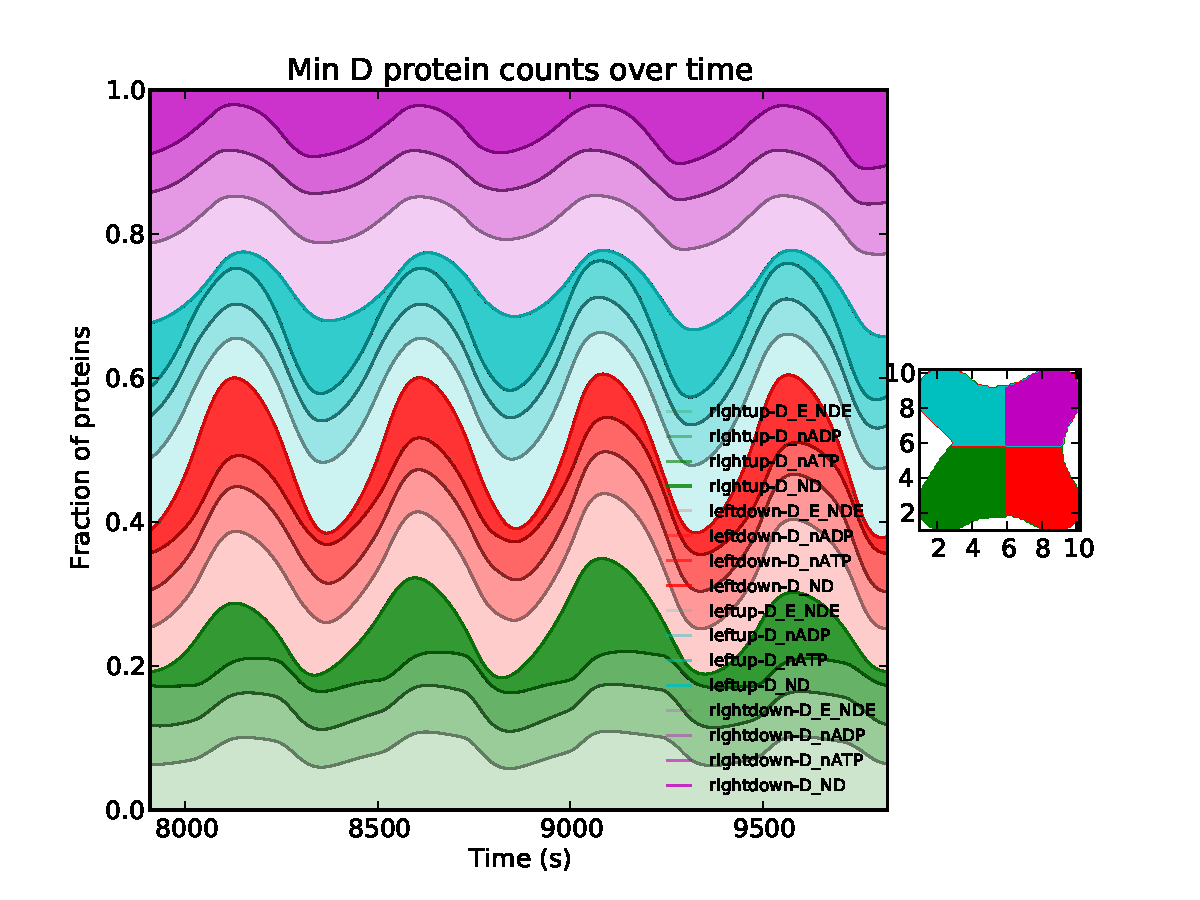
\includegraphics[width=\columnwidth]{../data/shape-randst/plots/box-plot_D--randst-25-600-600-9600-1500}
%%   \caption{Total protein fluctuation in the sideways flying saucer
%%     pancake cell shape.  The vertical axis shows stacked the total
%%     number of proteins that are of four different compound stages and
%%     in the different sections of the cell.}
%%   \label{box-97}
%% \end{figure}

%% Early on in its simulation the sideways flying saucer pancake shape
%% shows a clear breakdown of an unstable equilibrium oscillation.  We
%% have set the intial conditions so that MinD density is highly
%% concentrated to the left of a dividing line that runs parrallel to the
%% left vertical side.  For the first number of oscillations the maxima
%% trade off right to left, from a high peak in the rightward middle
%% compartment to vertically opposed peaks in the poles of the long axis
%% of the cell.  This is seen in the first part of Figure~\ref{box-97},
%% where the lower and upper sections peak in unison, and the middle
%% right section peaks $\pi$ radians removed from these.  After a few
%% oscillations the back and forth oscillations tip toward the vertical
%% direction and the system loses its initial oscillation pattern.  It
%% falls quickly instead into a back and forth pattern between the two
%% opposing endcaps.  The oscillation at this point is reminiscent of the
%% pills shape oscillation, once again showing the robust nature of the
%% back and forth, two pole pattern.

%% During each period, directly after one of the polar maxima has
%% subsided, there is a small spike with the regular maxima pattern (a
%% spike in membrane bound MinD:ATP immediately followed by a spike in
%% membrane bound MinD:MinE:ATP) seen in the small middle right
%% compartment section.  The animations show that the MinD, oscillating
%% back and forth between the upper and lower poles, seems to catch and
%% lag in the indentation for a bit before moving on.  Once again the
%% positive radius of curvature acts as an attractive place for MinD to
%% cluster on the walls, and it is not released to move on through the
%% cytoplasm again until MinE has formed its ring and completely reacted
%% it away.


%% \subsubsection{Randst-96-Star}
%% \begin{figure}
%%   \includegraphics[width=\columnwidth]{../data/shape-randst/plots/box-plot_D--randst-25-700-700-9600-1500}
%%   %%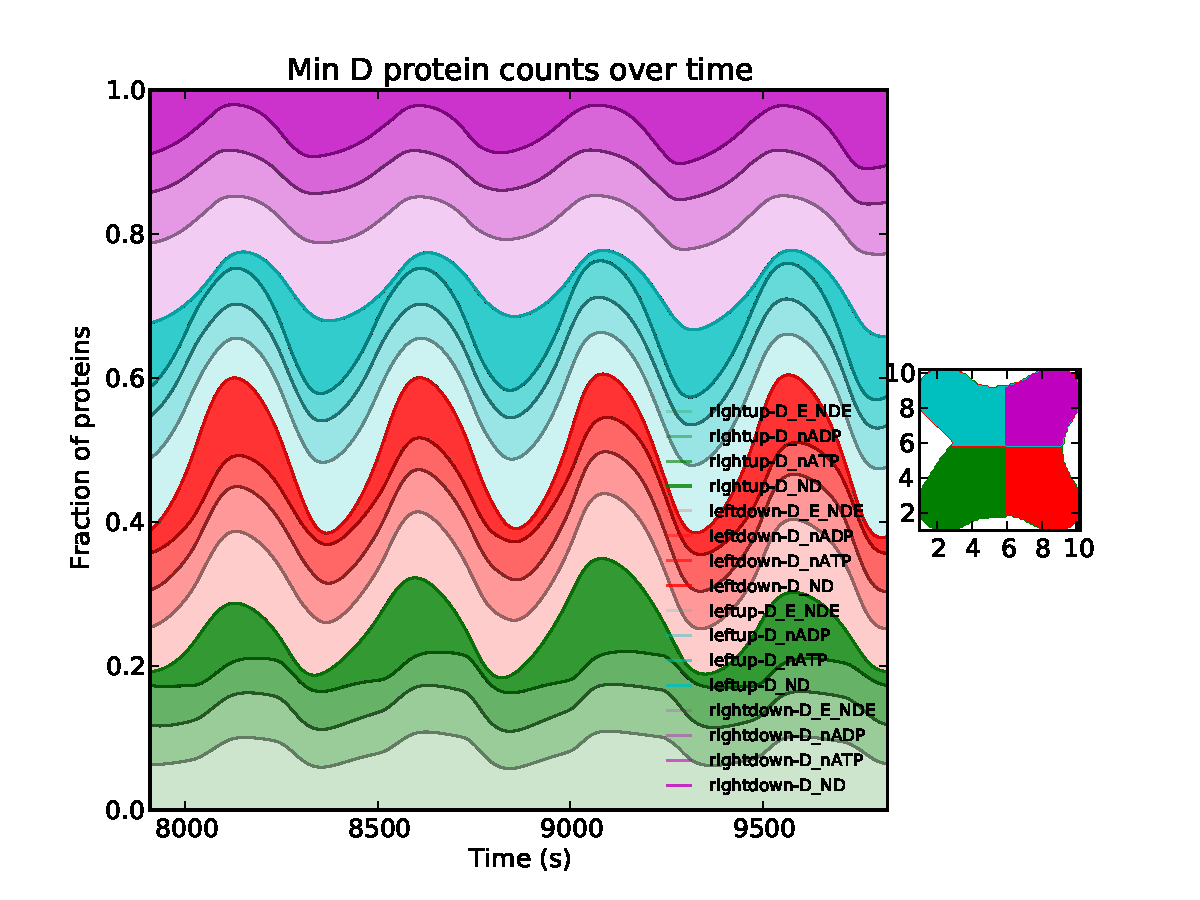
\includegraphics[width=\columnwidth]{../data/shape-randst/plots/box-plot_D--randst-25-600-600-9600-1500}
%%   \caption{Total protein fluctuation in the star cell shape.  The vertical axis shows stacked the total
%%     number of proteins that are of four different compound stages and
%%     in the different sections of the cell.}
%%   \label{box-96}
%% \end{figure}

%% This clover shape finds a regular oscillatory behavoir after about
%% seven periods that consists of two maxima that peak regularly in the
%% corners accross from each other at the same times (Figure
%% \ref{box-96}) and then again opposing maxima that peak at the same
%% time in the other two corners.\fixme{should try some different
%%   starting conditions with this to see if there's another patter.}

%% Looking at at few periods in detail.  We find that there is a small
%% increase in cytoplasmic MinE always directly before the beggining
%% of climb in the membrane bound MinE peak.  Also, there is at any one
%% time a very large amount more of minE that is membrane bound then
%% cytoplasmic in any ones section.  A difference of a factor of roughly
%% 20 when membrane MinE is at its peak, and roughly 12 when membrane
%% MinE is at it's minimum.  There seem to be two modes of oscillation,
%% each exhibiting a density peak maxima that moves back and forth
%% diagonaly from one corner to the opposite, as if there were two
%% overlapping, criss-crossed cells oscillating.  In the box plot this is
%% seen as roughly coinciding membrane minD peaks in the lower left and
%% right corners, followed one pi later in peaks in the upper right and
%% upper left corners.  Interesting that this did not exhibit
%% counterclockwise motion that Huangs 2008 paper might suggest.  Should
%% run sims that start in the wacky way that just started running with
%% triangles.
%% \newline


%% We haven't simulated long enough yet, so no real pattern has shown
%% itself.  There's certainly oscillations, and it's almost as if there's
%% competing modes - top to bottom, left to right, corner to corner, etc.
%% Interesting.

%% \fixme{maybe?}The animations seem to relax into a pattern in which the oscillations
%% go from the smallest corner, out to the other three, and then back to
%% the smallest corner?  \fixme{There isn't enough data to see properly
%%   though, need to run for longer.}

%% The double pole oscillation pattern, in which one pole is located in a
%% single corner of the triangle and the other pole is spread out between
%% the opposite two, can be seen in Figure \ref{box-triangle}.  The
%% equilateral triangle shows a spike in both the Center and Left
%% sections at the same time, both showing the familiar sequence of peaks
%% amoungst the different states of the protein seen in the poles of the
%% pill shaped bacteria.  A spike in the other corner, showing the common
%% sequence, occurs during the minima of the former two, wth a higher
%% concentration at the peak.  A similar pattern is seen in the
%% iscosolese triangular shape, where interestingly the onset of the
%% maxima in the single maxima corner (the Left section) builds more
%% quickly than it fades.  This is presumably becuase as the cytoplasmic
%% minD:ATP diffuses down a more accute corner, it is sourrounded by
%% closer cell walls than it would be in a less acute corner, so that the
%% it is more apt at any diffusive step to make contact and cluster on
%% the walls.  That particular part of the process is therefore
%% accelerated, driving the build up of the maxima forward.

%% The right triangle shows a similar pattern except that here there is
%% an assymetry between the two corners that maximize at roughly the same
%% time.  One corner is further from the single maximizing corner and it
%% consisitently peaks later.  The MinD simply have further to travel
%% before they maximize there.

%% For these three sizess and shapes there is not sign that the
%% oscillation patterns once they are set will break down.

%% \begin{figure}
%% %%  \includegraphics[width=\columnwidth]{../data/shape-triangle/plots/box-plot_D--triangle-25-600-600-600-1500}
%%   \caption{Total protein fluctuation of an equilateral triangle with
%%     larger dimensions (each side is roughly $6\micron$.  The vertical
%%     axis shows stacked the total number of proteins that are of four
%%     different compound stages and in the different sections of the
%%     cell. The time limits have been set to show the broken down
%%     section of the simulation.}
%%   \label{box-triangle}
%% \end{figure}

%% The larger equilateral shape shows the same pattern as the smaller
%% version does only until fifteen periods, at which point there is a
%% breakdown of the oscillation pattern.  During the last three stable
%% periods, the single maximizing corner, the lower left section in the
%% figure, has a lower peak each period as the membrane bound MinD:ATP in
%% the other corners lag more and more before being eaten away by the
%% MinE.  Finally these maxima lag so much that they break down the
%% regular pattern.  There then occurs about five periods of semi chaotic
%% behavoir, until it settles back into another stable oscillation that
%% is similar to the original one, except that a different corner has
%% been chosen to be the singlular maxima (the right section in the
%% figure), while the other two corners maximize at the same time.  This
%% interesting breakdown and recovery shows both the robustness of the
%% double pole oscilatory tendency and the importance of required
%% distance of travel for the different proteins.



\end{document}
